\subsection{Rechteckiger Stab, einseitig eingespannt} \label{sec:auswertung_einseitig_rechteckig}
Zunächst wurde eine Masse entsprechend der gewünschten Durchbiegung gewählt und fünfmal gewogen.
Es ergab sich eine mittlere Masse von \SI{1006.100 \pm 0.405}{\gram}.

\begin{table}
\centering
\caption{Wiederholte Messung des benutzten Gewichts.}
\begin{tabular}{S}
\toprule
$m \mathbin{/} \si{\gram}$ \\
\midrule
1005.9 \\
1006.9 \\
1005.8 \\
1005.9 \\
1006.0 \\
\bottomrule
\end{tabular}
\end{table}


In \autoref{tab:durchbiegung1} sind die Durchbiegung ohne Last ($D_\text{0}$), unter Last ($D_\text{M}$) und die tatsächliche Durchbiegung ($D$) mit der Position der Messuhr ($x$) aufgelistet.

\begin{table}
\centering
\caption{Durchbiegung des rechteckigen Stabes nach $x$-Abstand.}
\label{tab:durchbiegung1}
% \sisetup{table-format=2.1}
\begin{tabular}{c c c c}
\toprule
$x \mathbin{/} \si{\centi\meter}$ &
$D_0 \mathbin{/} \si{\micro\meter}$ &
$D_\text{M} \mathbin{/} \si{\micro\meter}$ &
$D \mathbin{/} \si{\micro\meter}$ \\
\midrule
\expandableinput{build/table_einseitig_eckig.tex}
\bottomrule
\end{tabular}
\end{table}

\FloatBarrier

Es wurde $D(x)$ gegen den Linearisierungsterm $Lx^2-\frac{x^3}{3}$ aufgetragen (siehe \autoref{fig:regression1})
und mithilfe von NumPy eine Regressionsgerade $D(x) = k_1 \cdot x + c_1$ berechnet.
Deren Parameter sind:
\begin{align*}
  k_1 &= \SI{0.00309 \pm 0.00011}{\meter\tothe{-2}} \\
  c_1 &= \SI{-0.020 \pm 0.006}{\milli\meter} \; .
\end{align*}

Das Flächenträgheitsmoment $\mathbf{I}$ lässt sich durch \autoref{eqn:I_rechteckig} mit den Abmessungen aus \autoref{sec:abmessungen} zu
$\mathbf{I} = \SI[{scientific-notation = true, separate-uncertainty = true}]{1.431(9)e-9}{\meter\tothe{4}}$ bestimmen.

Die Gewichtskraft $F_G = g \cdot m$ ist durch die Erdbeschleunigung und die zuvor bestimmte Masse gegeben.

Schließlich ist
\begin{equation*}
  E
  = \frac{F_G}{2 k_1 \mathbf{I}}
  % Welch unintuitive Schreibweise! :/
  = \SI[{scientific-notation = true, separate-uncertainty = true}]{4.65(17)e4}{\newton\per\square\milli\meter}
\end{equation*}
der gesuchte Elastizitätsmodul.

Die Messunsicherheit des Elastizitätsmoduls lässt sich gemäß der Gaußschen Fehlerfortpflanzung nach
\begin{equation*}
  \symup{\Delta}E = \frac{\partial E}{\partial m} \cdot \symup{\Delta}m
\end{equation*}
berechnen.

\begin{figure}
  \centering
  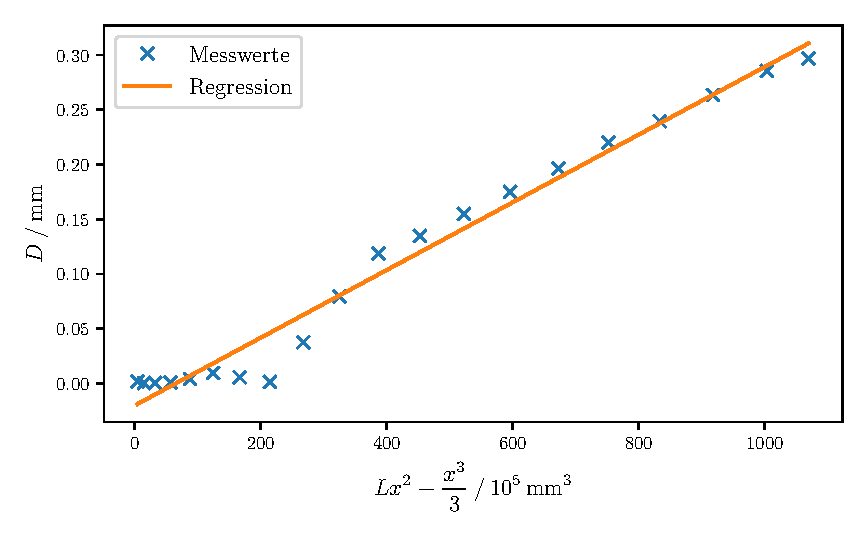
\includegraphics[scale=0.8]{build/plot_einseitig_eckig.pdf}
  \caption{Durchbiegung eines einseitig eingespannten eckigen Stabes, aufgetragen gegen einen Linearisierungsterm.}
  \label{fig:regression1}
\end{figure}
